
%%% Local Variables:
%%% mode: latex
%%% TeX-master: "master"
%%% End:



\chapter{Background}

\section{Formal System}

A formal system is any well-defined system of abstract thought based on mathematical model\supercite{formal-system-wiki}. Each formal system has a formal language composed of primitive symbols\footnote{phometa will assume that primitive symbols are any Unicode character.} acted by certain formation\supercite{formal-system-britannica}.

% For example, propositional logic has a grammar like this


% If not stated otherwise, phometa will assume that primitive symbols are all of unicode,

% Since phometa aims to be a tool and can create arbitrary formal system. So syntax and derivation rule part are vital as well. We try In fact, most of preliminary
% Although proof assistant related mainly on proving mechanism but we
% If we keep thinking


%  Formally proving a line of proposition might need a page of derivation tree. This is worse than its sound since the width of a tree grows exponentially to its height.


% Many of formal systems such as first-order logic\footnote{First-order logic is a logical system, but we can see it as formal system by exclude semantics part.} and lambda calculus are considered to be the most fundamental components Mathematics and Computer Science. Each of them has been designed and implemented separately, however, these formal systems have something in common, for examples,

% \begin{itemize}
%   \item first-order logic consists of
%   \begin{itemize}%[label={}]
%       \item \textbf{Syntax} Grammars of propositions, atoms, terms, variables, etc.
%       \item \textbf{Reductions} How to reduce complex proposition into simpler one, how to define substitution, etc.
%       \item \textbf{Proof Rules} $\wedge$-intro, $\wedge$-elim, $\rightarrow-intro$, $\rightarrow$-elim, etc.
%       \item \textbf{Theorems} T
%   \end{itemize}
%   \item lambda calculus consists of
%   \begin{itemize}%[label={}]
%       \item \textbf{Syntax} Grammars of propositions, atoms, terms, variables, etc.
%       \item \textbf{Reduction} How to reduce complex proposition into simpler one, how to define substitution, etc.
%       \item \textbf{Proof Rules} $\wedge$-intro, $\wedge$-elim, $\rightarrow-intro$, $\rightarrow$-elim, etc.
%   \end{itemize}
% \end{itemize}

% Since


\section{Natrual Deduction}

\section{Big picture --- Formal Verification}
Formal Verification is one of major topics in Computer Science. It dealing with proving or disproving the correctness of algorithms used in curtain system\supercite{formal-verification-wiki}  which is necessary for some critical applications such as rocket launcher or medical surgery where bugs in programs can cause lose of life or financial crisis.

Formal Verification itself split into two ends of spectrum, Model Checking and Theorem Proving. Model Checking required a complete formal-specification of the system, then it will automatically tell us weather the curtain property holds or not. Theorem Proving, in the another hand require us to proof the by our self with some part become automatic if possible.

These two ends of spectrum doesn't superior to one another. Model Checking is easier to used than Theorem Proving (since everything is completely automatic) whereas Theorem Proving has wider horizon of provable properties (since users can give move specific hint on particular property).

Phometa takes Theorem Proving approach with some part become automatic.

\section{Related Traditional Proof Assistant}

\subsection{Coq}
Coq\supercite{coq-official-website} is one the most famous interactive theorem prover. Coq works within the theory of the calculus of inductive constructions (CIC)\footcite{CIC is itself is developed alongside Coq.} developed by Thierry Coquand\supercite{thierry-coquand-homepage}. Its proving technique relies mainly on tactics which are commands that tell Coq how to prove particular theorem, this might look confuse at the first time but comes to handy later especially when we want to prove something complex.

\begin{figure}[H]
    \centering
    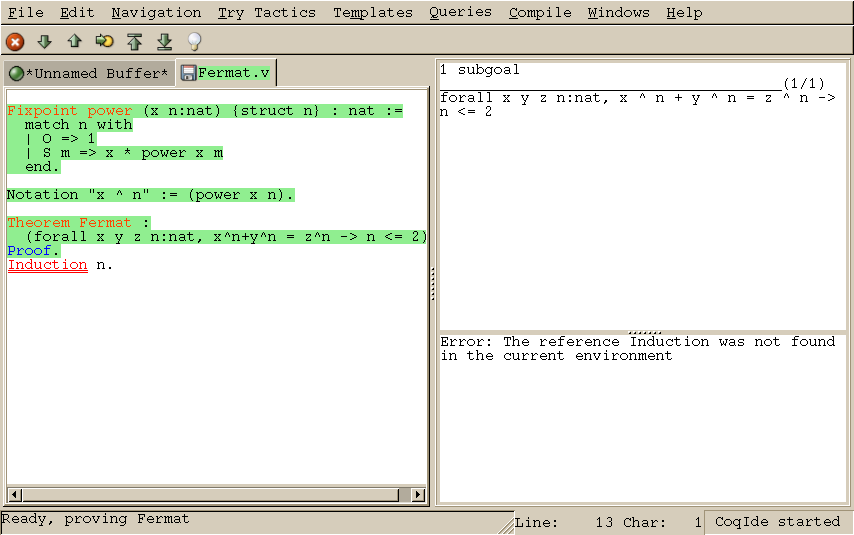
\includegraphics[width=\textwidth]{background-coq}
    \caption{Coq in action --- with CoqIDE \supercite{coq-official-website}}
\label{fig:background-coq}
\end{figure}

\subsection{Agda}
Adga\supercite{agda-official-website} is (dependent type) functional programming which can be seen as a proof assistant as well. It is based on Martin Lof Type Theory\footnote{CIC is an impredicative version of Martin Lof Type Theory}. Its proving technique is relies on Curry-Howard correspondence which state that there is direct relationship between computer programs and mathematical proofs\supercite{curry-howard-correspondence}, for example function corresponded to logical implication, product type corresponded to logical implication.

\subsection{Lean}
Lean\supercite{lean-offical-website} is a relatively new theorem prover\footnote{The Lean project was launched by Leonardo de Moura at Microsoft Research in 2013}

\section{Related Visualised Proof Assistant}
Sorry I can't finish some part of background chapter for interim report, this will be done in later version.

\subsection{Pandora}
\subsection{http://logitext.mit.edu/tutorial}
\subsection{Why3}
